\documentclass[a4paper]{article}
\usepackage{amsmath}
\usepackage{amssymb}
\usepackage{geometry}
\usepackage{enumerate}
\usepackage{natbib}
\usepackage{float}%稳定图片位置
\usepackage{graphicx,subfig}%画图
\usepackage{caption}
\usepackage[english]{babel}
\usepackage{indentfirst}%缩进
\usepackage{enumerate}%加序号
\usepackage{multirow}%合并行
\usepackage{hyperref}
\hypersetup{hypertex=true, colorlinks=true, linkcolor=black, anchorcolor=black, citecolor=black}
\title{\Large \textbf{VP390 Problem Set 2}\\
\author{\textbf{Pan, Chongdan ID:516370910121}\\
}
}
\begin{document}
\maketitle
\section{Problem 1}
\begin{enumerate}[(a)]
    \item $m(u^2)=\frac{m}{\sqrt{1-u^2/c^2}}=\sqrt{3}m$
    \\Since $m_{ij}=m(u^2)[\delta_{ij}+\frac{1}{c^2-u^2}u_iu_j]=\sqrt{3}m(\delta_{ij}+\frac{3}{c^2}u_iu_j)$
    \\Then $mij=\sqrt{3}m\left(                
    \begin{array}{ccc}   
      1+1 & 0 & 1\\ 
      0 & 1 & 0\\  
      1 & 0 & 1+1\\  
    \end{array}
    \right)=\sqrt{3}m\left(
    \begin{array}{ccc}   
        2 & 0 & 1\\ 
        0 & 1 & 0\\  
        1 & 0 & 2\\  
      \end{array}
  \right) $
  \item $F=ma=\sqrt{3}m\left(\begin{array}{ccc}   
    2 & 0 & 1\\ 
    0 & 1 & 0\\  
    1 & 0 & 2\\  
  \end{array}\right)\left(\begin{array}{ccc}   
    0\\ 
    0\\  
    1\\  
  \end{array}\right)=\sqrt{3}m\left(\begin{array}{ccc}   
    1\\ 
    0\\  
    2\\  
  \end{array}\right)$
  \begin{figure}[H]
    \centering
    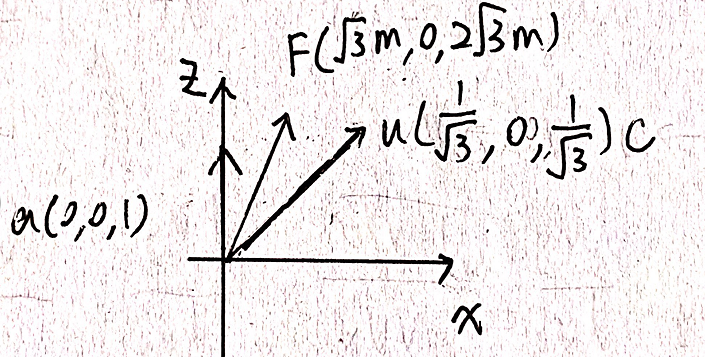
\includegraphics[scale=0.25]{P1.png}
    \caption{The y component is all 0, so the plot only show the x-z plane}
    \label{P1}
\end{figure}

\end{enumerate}
\section{Problem 2} 
\quad 
\\$E^2=p^2c^2+E_0^2$ where $E_0=mc^2$
\\Since $p=p_1,E=E_1+E_2$
\\Then $m^2=m_1^2+m_2^2$
\\So the new particle's rest mass m is $\sqrt{m_1^2+m_2^2}$
\\$E=K_1+m_1c^2+m_2c^2=\frac{mc^2}{\sqrt{1-u^2/c^2}}$
\\Then the new particle's velocity is $c\sqrt{1-\frac{m_1^2c^4+m_2^2c^4}{(K_1+m_1c^2+m_2c^2)^2}}$
\section{Problem 3}
\quad
\\If it's possible, then the total energy for the electron after collision is :
\\$E_{electron}=E_{photon}+E_{0}$ where $E_0=mc^2$
\\For the momentum $p=\frac{E_{photon}}{c}$
\\Since $E^2=p^2c^2+E_0^2$
\\Then $E_{electron}=\sqrt{E_{photon}^2+E_{0}^2}\neq E_{photon}+E_{0}$
\\So it's impossible.
\section{Problem 4}
\quad
\\$L_z=n^2\hbar^2$
\\$L_{\mathrm{ph}}=n'^2\hbar^2-n^2\hbar$
\section{Problem 5}
\quad
\\$R(\lambda)=\frac{1}{4}cu(\lambda)=\frac{2\pi}{\lambda^5}\frac{hc^2}{e^{hc/\lambda k_\mathrm{B}T}-1}$
\\Let $R(\lambda)'=0$, we can get $\frac{2c^3h^2\pi e^{ch/k_\mathrm{B}T\lambda}}{(-1+e^{ch/k_\mathrm{B}T\lambda})^2 k_\mathrm{B}T\lambda^7}-\frac{10c^2h\pi}{(-1+e^{ch/k_\mathrm{B}T\lambda})\lambda^6}=0$
\\Ignore the root where $\lambda=0$ we can get $\frac{che^{ch/k_\mathrm{B}T\lambda}}{(-1+e^{ch/k_\mathrm{B}T\lambda})\lambda k_\mathrm{B}T}=5$
\\Let $x=\frac{ch}{k_\mathrm{B}T\lambda}$ we get $\frac{xe^x}{e^x-1}=5$
\\The solution $x\approx4.96$, so $\lambda_mT=\frac{xk_\mathrm{B}}{ch}\approx2.9\times10^{-3}(m\cdot K)$
\section{Problem 6}
\begin{enumerate}[(a)]
    \item \quad
    \\Since $\lambda_2-\lambda_1=\frac{h}{mc}(1-\cos\theta)$
    \\Then $\frac{c}{\nu_2}=\frac{h}{mc}(1-\cos\theta)+\frac{c}{\nu}$
    \\The energy of scattered photon is $h\nu_2=\frac{hc}{\frac{h}{mc}(1-\cos\theta)+\frac{c}{\nu}}=\frac{hm\nu c^2}{h\nu+mc^2-h\nu\cos\theta}$
    \\\\For the electron, the total energy will be $E_e=h\nu+mc^2-h\nu_2$, and $K_c=E_e-mc^2=h\nu-h\nu_2$
    \\$K_c=E_e-mc^2=h\nu(1-\frac{mc^2}{h\nu+mc^2-h\nu\cos\theta})$
    \\When $\cos\theta=-1$, we can get the max $K_c=\frac{h\nu}{1+\frac{mc^2}{2h\nu}}$
    \item \quad
    \\$K_c=\frac{2E^2}{2E+mc^2}$, then $2E^2-2EK_c-mc^2K_c=0$
    \\$E=\frac{2K_c\pm\sqrt{4K_c^2+8mc^2K_c}}{4}$, keep the positive solution we can get 
    \\$E=1.133\times10^{-13}J$
    \\$\lambda=\frac{c}{\nu}=\frac{hc}{E}=1.75\times10^{-12}m$
\end{enumerate}
\section{Problem 7}
    \quad
    \\$\Psi_{12}=|\Psi_1+\Psi_2|^2=|\Psi_1|^2+|\Psi_2|^2+2\mathrm{Re}(\Psi_1\Psi_2^*)$
    \\$\Psi_1=\frac{1}{\sqrt{2}}e^{-\frac{y^2}{2}}\cos(\omega t-ay)+\frac{1}{\sqrt{2}}e^{-\frac{y^2}{2}}\sin(\omega t-ay)i$
    \\$\Psi_1=\frac{1}{\sqrt{2}}e^{-\frac{y^2}{2}}\cos(\omega t-ay-by)+\frac{1}{\sqrt{2}}e^{-\frac{y^2}{2}}\sin(\omega t-ay-by)i$
    \\$|\Psi_1|^2=|\Psi_2|^2=\frac{e^{-y^2}}{2}$
    \\$\mathrm{Re}(\Psi_1\Psi_2^*)=\frac{e^{-y^2}}{2}\cos(\omega t-ay)\cos(\omega t-ay-by)+\frac{e^{-y^2}}{2}\sin(\omega t-ay)\sin(\omega t-ay-by)$
    \\$\mathrm{Re}(\Psi_1\Psi_2^*)=\frac{e^{-y^2}}{2}\cos by$
    \\$\Psi_{12}=e^{-y^2}(1+\cos by)$
\end{document}